\section{Study overview}
\newcommand{\RNum}[1]{\uppercase\expandafter{\romannumeral #1\relax}}
Studie \RNum{1} var å teste om reinforcement learning er en bedre læringsstrategi for å hjelpe utøvere til å ta gode strategivalg sammenlignet med tradisjonell coaching instruksjon (supervised learning). For å teste dette designet vi en læringsintervensjon som gikk over tre dager. I læringsintervensjonen brukte vi et between-subjects design og multi-armed bandit.  Studie \RNum{2} besvarte hvilke av disse strategiene som utøverne presterte best med. 


\begin{figure}[H]
\centering
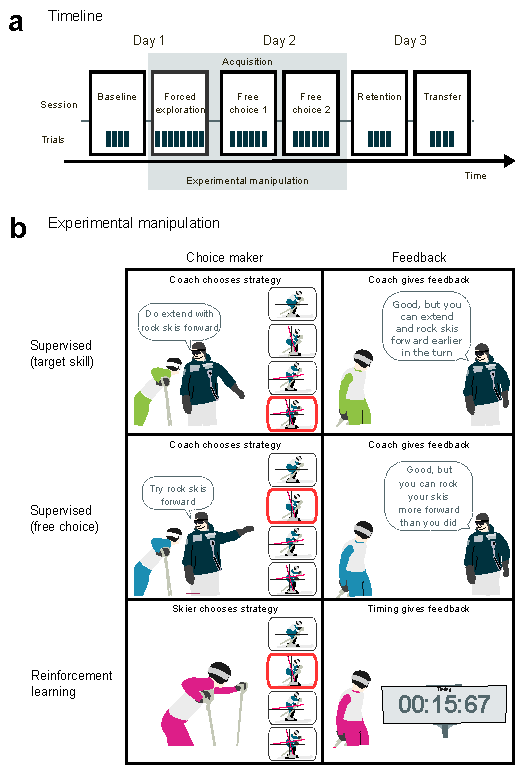
\includegraphics{figure_method_experiment.pdf}
\caption{Acceleration in the local positioning system section.\textbf{a.} Estimated acceleration during baseline and retention for the local positioning section. \textbf{b}. Expected mean difference between baseline and retention in the local positioning section.\textbf{c.} Estimated total gate-to-gate acceleration during baseline and retention in the local positioning section. \textbf{d}. Expected mean difference between baseline and retention in the local positioning section. The black lines denote the expected mean or differences in mean, with the shaded area representing their 95\% credible interval (CI). Each gray point or line represents one run trial by a skier}\label{fig: acc}
\end{figure}


\section{Setup}

